% -*- TeX:de -*-
\NeedsTeXFormat{LaTeX2e}
\documentclass[12pt,a4paper]{article}
\usepackage[german]{babel} % german text
\usepackage[DIV12]{typearea} % size of printable area
\usepackage[T1]{fontenc} % font encoding
%\usepackage[latin1]{inputenc} % most likely on Windows
\usepackage[utf8]{inputenc} % probably on Linux
\usepackage{multicol}

% PLOTTING
\usepackage{pgfplots} 
\usepackage{pgfplotstable}
\usepackage{url}
\usepackage{graphicx} % to include images
\usepackage{tikz}
\usepackage{subfigure} % for creating subfigures
\usepackage{amsmath} % a bunch of symbols
\usepackage{amssymb} % even more symbols
\usepackage{booktabs} % pretty tables
\usepackage{makecell} % multi row table heading

% a floating environment for circuits
\usepackage{float}
\usepackage{caption}

%\newfloat{circuit}{tbph}{circuits}
%\floatname{circuit}{Schaltplan}

% a floating environment for diagrams
%\newfloat{diagram}{tbph}{diagrams}
%\floatname{diagram}{Diagramm}
\pgfplotsset{compat=1.8}
\selectlanguage{german} % use german

\begin{document}

%%%%%%% DECKBLATT %%%%%%%
\thispagestyle{empty}
			\begin{center}
			\Large{Fakultät für Physik}\\
			\end{center}
\begin{verbatim}


\end{verbatim}
							%Eintrag des Wintersemesters
			\begin{center}
			\textbf{\LARGE SS 14}
			\end{center}
\begin{verbatim}


\end{verbatim}
			\begin{center}
			\textbf{\LARGE{Physikalisches Praktikum\\ für das Bachelorstudium}}
			\end{center}
\begin{verbatim}




\end{verbatim}

			\begin{center}
			\textbf{\LARGE{PROTOKOLL}}
			\end{center}
			
\begin{verbatim}

\end{verbatim}

			\begin{flushleft}
			\textbf{\Large{Experiment (Nr., Titel): PS11 - Halleffekt in dotierten Halbleitern}}\\
							%Experiment Nr. und Titel statt den Punkten eintragen
			\LARGE{PS11 }	
			\end{flushleft}

\begin{verbatim}

\end{verbatim}	
							%Eintragen des Abgabedatums, oder des Erstelldatums des Protokolls
			\begin{flushleft}
			\textbf{\Large{Datum:}} \Large{15.05.2014}
			\end{flushleft}
			
\begin{verbatim}
\end{verbatim}
							%Namen der Protokollschreiber
		\begin{flushleft}
			\textbf{\Large{Namen:}} \Large{Patrick Braun, Johannes Kurz}
			\end{flushleft}

\begin{verbatim}


\end{verbatim}
							%Kurstag und Gruppennummer, zb. Fr/5
			\begin{flushleft}
			\textbf{\Large{Kurstag/Gruppe:}} \Large{DO/4}
			\end{flushleft}

\begin{verbatim}

\end{verbatim}
							%Name des Betreuers, das Praktikum betreute.
			\begin{flushleft}
			\LARGE{\textbf{Betreuer:}}	\Large{Wilhelm Markowitsch}	
			\end{flushleft}

%%%%%%% DECKBLATT ENDE %%%%%%%
\pagebreak
\setlength{\columnsep}{20pt}
\begin{multicols}{2}

%%%%%%%%%%%%%%%%%%%%%%%%%%%%%%%%%%%%%%%%%%%%%%%%

%\begin{figure}[H]
%	\centering
%	\includegraphics[scale=0.35]{./data/beugung.png}
%	\caption{Beugungsmuster Einzelspalt (echtes Foto; schwarz durch weiß ersetzt)}
%	\label{fig:beugungsmuster}
%\end{figure}


%\begin{figure}[H]
%	\centering
%	\pgfplotstabletypeset[
%			columns={abstand, n},
%			col sep=&,
%			columns/abstand/.style={precision=2, zerofill, column name=\makecell{$Abstand$\\$(\pm 0.05)[mm]$} }, 
%			columns/n/.style={column name=\makecell{$n$\\$(Ordnung)$}, precision=0},
%			every head row/.style={before row=\hline,after row=\hline\hline},
%			every last row/.style={after row=\hline},
%			every first column/.style={column type/.add={|}{} },
%			every last column/.style={column type/.add={}{|} }
%			]{
%			abstand & n
%			12.9 & 1
%			24.45 & 2
%			37.40 & 3
%			49.35& 4
%			62.45 & 5
%			74.45 & 6
%			87.45 & 7
%			100.25 & 8
%			
%			}
%	\caption{Messwerte Einzelspalt}
%	\label{tab:werte_einzelspalt}
%\end{figure}


%%%%%%%%%%%%%%%%%%%%%%%%%%%%%%%%%%%%%%%%%%%%%%%%
%%%%%%%%%%%%%%%%%%%%%%%%%%%%%%%%%%%%%%%%%%%%%%%%

In diesen Experimenten werden die Eigenschaften von dotierten Halbleitern in Bezug auf den Hall-Effekt untersucht. Der Hall-Effekt ist das Auftreten einer Spannung normal stehend zur Flussrichtung eines an den Halbleiter angelegten Stromes.\\


\section{Hall-Effekt in n- und p-dotiertem Germanium}
Im Halbleiter aus Germanium wird im Folgenden der lineare Zusammenhang zwischen Strom und Hallspannung überprüft.

\subsection{Grundlagen}
Grundlage der Hallspannung ist die Lorenzkraft. In ([1] p. 5 Abb. 2) ist der Aufbau der Untersuchung wie folgt zu sehen:

\begin{figure}[H]
	\centering
	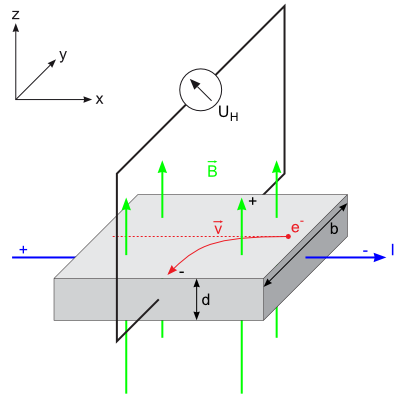
\includegraphics[scale=0.5]{./figures/hallspannung_aufbau.png}
	\caption{Entstehung der Hallspannung $U_H$ an einem stromdurchflossenen Leiter in einem Magnetfeld B.}
	\label{fig:hallspannung_aufbau}
\end{figure}

Hier ist zu sehen das normal zur Stromrichtung (in z-Richtung) das Magnetfeld angelegt wird. Normal zu Stromrichtung und normal zum Magnetfeld (Kreuzprodukt) liegt die Hallspannung an. Wie bereits erwähnt ist der Grund dafür die Lorenzkraft:

$$\vec{F_{L}} = q \cdot \vec{E} + q \cdot (\vec{v} \times \vec{B})$$



\subsection{Versuchsaufbau}





\end{multicols}
\subsection{Resultate}

%nGe UH-B
%Von x = -2,199292000000000e-01 bis x = 2,180299000000000e-01
%B (y-intercept) = 4,662737519668038e-04 +/- 1,508714424821067e-04
%A (slope) = 2,248372979857526e-01 +/- 1,124478213531423e-03
%--------------------------------------------------------------------------------------
%Chi^2/doF = 4,324795635932366e-07
%R^2 = 0,999574960134199
%Angepasstes R^2 = 0,999521830150974
%RMSE (Standardabweichung) = 0,000657631784202404
%RSS (Summe der quadrierten Restwerte) = 7,35215258108503e-06
%---------------------------------------------------------------------------------------

%nGe -I UH
%Von x = 2,000000000000000e-03 bis x = 3,000000000000000e-02
%B (y-intercept) = -1,407260213143868e-03 +/- 9,794485115681493e-04
%A (slope) = -9,434502664298404e-01 +/- 5,428232838540915e-02
%--------------------------------------------------------------------------------------
%Chi^2/doF = 1,895908081705150e-06
%R^2 = 0,983717565353814
%Angepasstes R^2 = 0,975576348030721
%RMSE (Standardabweichung) = 0,00137691978041756
%RSS (Summe der quadrierten Restwerte) = 9,47954040852575e-06
%---------------------------------------------------------------------------------------

%nGe +I UH
%
%Von x = 2,000000000000000e-03 bis x = 3,000000000000000e-02
%B (y-intercept) = -1,544205222171330e-04 +/- 2,723794209658636e-04
%A (slope) = 7,535272560696289e-01 +/- 1,505932725754159e-02
%--------------------------------------------------------------------------------------
%Chi^2/doF = 1,414480073293634e-07
%R^2 = 0,998006956474477
%Angepasstes R^2 = 0,997010434711716
%RMSE (Standardabweichung) = 0,000376095742237749
%RSS (Summe der quadrierten Restwerte) = 7,07240036646817e-07
%---------------------------------------------------------------------------------------





\begin{figure}[H]
	\centering
	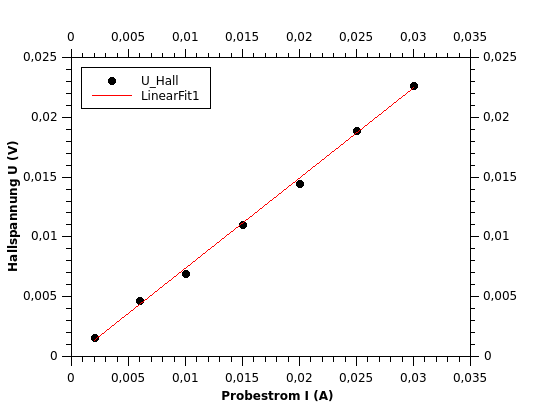
\includegraphics[scale=1.20]{./figures/Hall_nGe_+I_UH.png}
	\caption{Hallspannung mit Fit an einem n-dotierten Germaniumhalbleiter, mit positivem Strom}
	\label{fig:nGe_pI_UH}
\end{figure}
\begin{multicols}{2}



\end{multicols}
\begin{figure}[H]
	\centering
	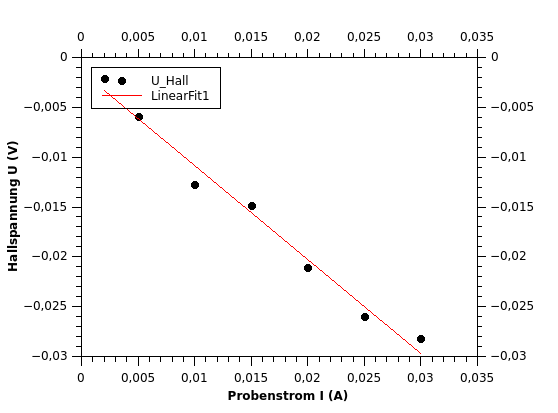
\includegraphics[scale=1.20]{./figures/Hall_nGe_-I_UH.png}
	\caption{Hallspannung mit Fit an einem n-dotierten Germaniumhalbleiter, mit negativem Strom}
	\label{fig:nGe_nI_UH}
\end{figure}
\begin{multicols}{2}



\end{multicols}
\begin{figure}[H]
	\centering
	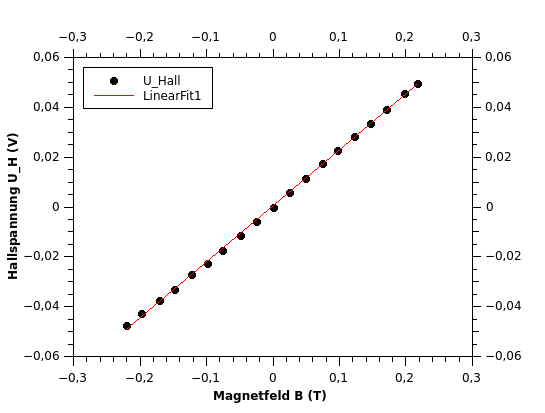
\includegraphics[scale=1.5]{./figures/Hall_nGe_UH-B.png}
	\caption{Hallspannung mit Fit bei variertem magnetischem Feld bei einem n-dotierten Germaniumhalbleiter}
	\label{fig:nGe_UH_B}
\end{figure}
\begin{multicols}{2}

\noindent \textbf{Hall-Effekt im n-Ge:}\\
Probendicke $d=1mm$\\
Strom/B-Feld Proportionalität:\\
$A=(48.70 \pm 0.25)\frac{mT}{A}$\\

\noindent \emph{positive Spannungsrichtung (Abb. \ref{fig:nGe_pI_UH}):}\\
$\frac{U_H}{I_{Probe}}=(0.754\pm 0.016)V/A$\\
$I_{B-Feld}=(2.031 \pm 0.001)A$\\
$$R_H=(7620 \pm 170)\frac{cm^3}{A\cdot s}$$
$$n=(8.1910\pm 0.019)\times 10^{14}cm^{-3}$$\\


\noindent \emph{negative Spannungsrichtung (Abb. \ref{fig:nGe_nI_UH}):}\\
$\frac{U_H}{I_{Probe}}=(-0.943\pm 0.016)V/A$\\
$I_{B-Feld}=(-2.059 \pm 0.001)A$\\
$$R_H=(9400 \pm 170)\frac{cm^3}{A\cdot s}$$
$$n=(6.6317\pm 0.13)\times 10^{14}cm^{-3}$$\\


\noindent \emph{negative Spannungsrichtung (Abb. \ref{fig:nGe_UH_B}):}\\
$\frac{U_H}{B}=(0.2248\pm 0.0012)V/T$\\
$I_{Probe}=(25 \pm 1)mA$\\
$$R_H=(8992 \pm 370)\frac{cm^3}{A\cdot s}$$
$$n=(6.9411\pm 0.29)\times 10^{14}cm^{-3}$$\\




\pagebreak
\end{multicols}
\noindent \textbf{Hall-Effekt im p-Ge:}\\



\begin{figure}[H]
	\centering
	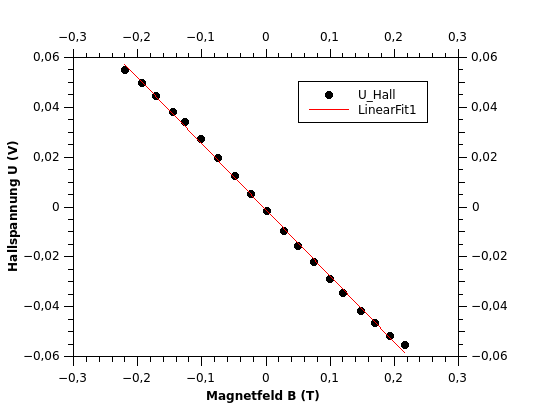
\includegraphics[scale=1.3]{./figures/Hall_pGe_UH-B.png}
	\caption{Hallspannung mit Fit bei variertem magnetischem Feld bei einem p-dotierten Germaniumhalbleiter}
	\label{fig:pGe_UH_B}
\end{figure}
\begin{multicols}{2}

Rohdaten sind zu finden unter [2].

\subsection{Diskussion}

\section{Temperaturabhängigkeit des Hall-Effekts}

\subsection{Grundlagen}

\subsection{Versuchsaufbau}

\subsection{Resultate}

%pGe Magnet UH
%Von x = 2,154975000000000e-01 bis x = -2,203675000000000e-01
%B (y-intercept) = -1,183992477161761e-03 +/- 3,331039840238531e-04
%A (slope) = -2,655354469324444e-01 +/- 2,493431990282161e-03
%--------------------------------------------------------------------------------------
%Chi^2/doF = 2,108132919598357e-06
%R^2 = 0,998503252811351
%Angepasstes R^2 = 0,998316159412769
%RMSE (Standardabweichung) = 0,0014519410868208
%RSS (Summe der quadrierten Restwerte) = 3,58382596331721e-05
%---------------------------------------------------------------------------------------
 




Rohdaten sind zu finden unter [2].

\subsection{Diskussion}


\section{Quellen}
$[1]$ Anleitung, \url{http://www.univie.ac.at/anfpra/neu1/ps/ps11/PS11.pdf}\\
$[2]$ Rohdaten, \url{htts://github.com/blackandcold/Protocols-SS2014-P2/tree/master/PS_11/daten}\\

\end{multicols}
\end{document}